\titleformat {\chapter} {\normalfont\huge\bfseries\color{black}}   {\thechapter}{10pt}{\huge} 
\chapter {Research Implementation Plan}

\section{Main Tasks in Research Implementation Plan}

The total estimated duration for this research project is 356 days or about 1 calendar year. As shown in the figure below, the project tasks have been separated into four main categories as follows:
\begin{enumerate}
	\item Project Preliminaries and Setup (Task No. 2 until Task No. 117)
	\item Software Design and Implementation (Task No. 146 until Task No. 178) 
	\item Software Testing and Reporting (Task No. 190 until Task No. 219) 
	\item Project Publication and Closing (Task No. 224 until Task No. 233) 
\end{enumerate}

\begin{figure}[htbp]
	\begin{center}
		\frame{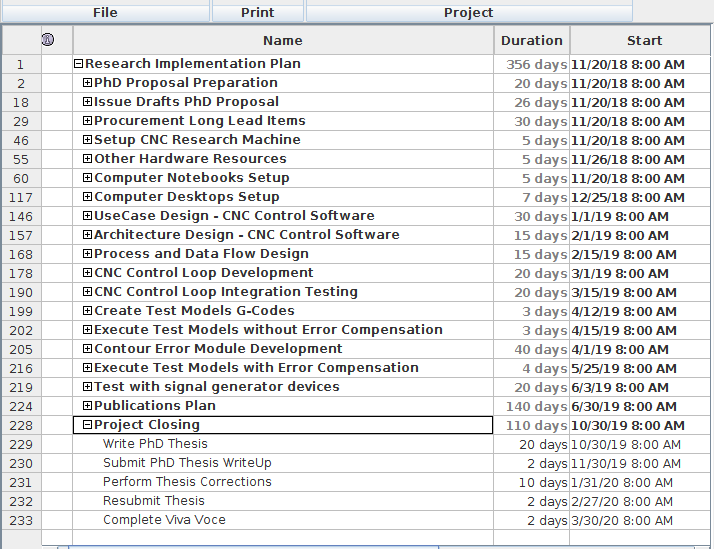
\includegraphics[width=0.95\textwidth]{./07-images/img-Ch5/00-Research-Implementation-Plan.png}}
		\caption{Main Tasks in Research Implementation Plan}
		\label{fig:00-Research-Implementation=Plan.png}
	\end{center}
\end{figure}

The Work Breakdown Structure (WBS) or subtasks with details for the Research Implementation Plan are provided in the appendix at the link Fig [~\ref{sec:App5-Research-Implementation-Plan}].

%%\vspace{0.5cm}
%%\vspace{0.5cm}

%% =================================================
\clearpage
\pagebreak
\begin{landscape}

\section{Overview of Research Implementation Schedule}

\begin{figure}[htbp]
	\begin{center}
		\frame{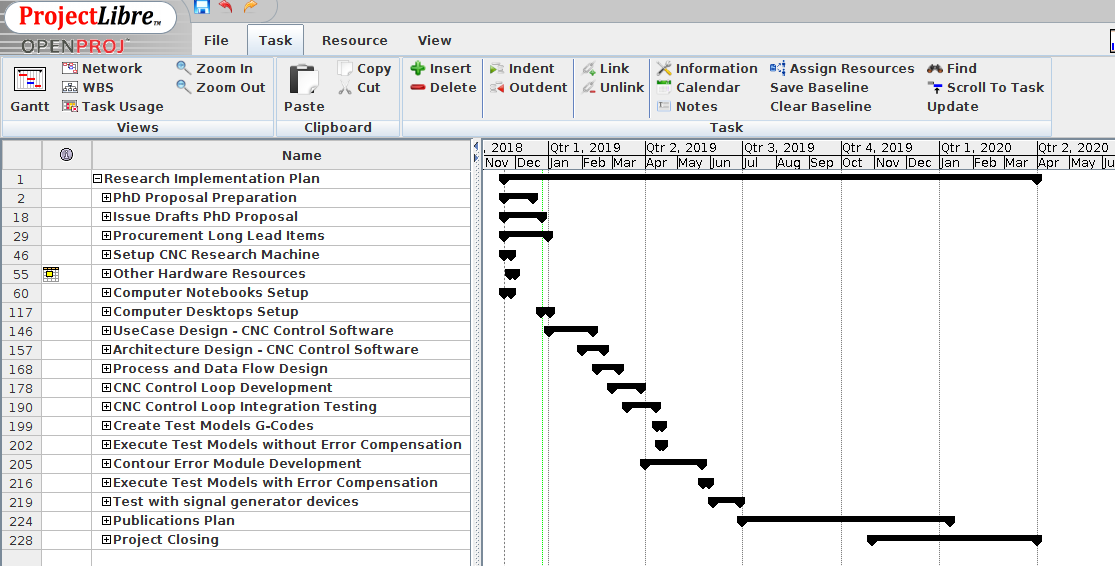
\includegraphics[width=1.35\textwidth]{./07-images/img-Ch5/Overview-Research-Implementation-Plan.png}}
		\caption{Overview of Research Implementation Schedule}
		\label{fig:Overview-Research-Implementation-Plan.png}
	\end{center}
\end{figure}

\end{landscape}

%% =================================================

\section{Critical Project Tasks} 
The identified critical tasks are the UseCase Design, Architecture Design, Process and Data Flow Design, and the Control Loop Design.
\vspace{0.5cm}

The UseCase design must be correct and complete covering all possibilities of system usage, link at [~\ref{sec:App5-UseCase Design}]. UseCases are the blueprint for software design. Incomplete UseCases may cause missing features and functions in the software. The software architecture, process flow, data flow and control loop designs, link at [~\ref{sec:App5-Process-Flow Design}], must ensure that the system will be built with flexible and upgradeable features. A design that is incomplete and rigid may require a complete design rework if certain new features need to be added or existing features need to be modified.	
\vspace{0.5cm}
	
Since software design is the blueprint for software construction, good design facilitates good software construction. In this project, we anticipate a few rounds of iterative designs since software construction will be conducted following the incremental and prototyping model. This software construction method saves time and eliminates complex logical design errors. In the incremental and prototyping model, the system is developed by starting from having small features, then incrementally built, tested, and then reworked as necessary until an acceptable complete system is achieved. This model works best where not all of the project requirements are known in detail ahead of time. This process development model is iterative, sort of, a trial-and-error process that repeats until the final design goals have been achieved. 
	
\section{Research Milestones}
The project milestones follow closely the project critical tasks. Successful completion of usecases, software architecture, process flow, data flow and control loop designs are the five primary milestones in this research project. Successful completion of control loop testing, integrated testing, hardware system testing and publication submissions are another four secondary milestones in this project.  
%% \vspace{0.5cm}
	
\section{Publications Plan}

We anticipate a total of three publications spread three months apart in this research project. The target is two conference publications and one journal publication. The first conference publication will be for the Pico Universal PWM hardware with LinuxCNC, and the second publication will be for the Microchip MCU Curiosity and 28-Pin LIN development boards and the CNC Control Software. The target journal publication will be for CNC Interpolation, which is the main thesis for this research.

% ======================================================	
\section{Implementation approach}
% ======================================================

The implementation approach is to focus on the utilization of modern software engineering technologies like efficient data structures, fast algorithms, realtime and parallel computations, tractable program executions, integrations of different programming language libraries and many more that will be explored during the software design stage. The final goal is to achieve an efficient implementation for a realtime and parallel look-ahead control and feedrate compensation strategy for CNC reference-pulse interpolation.

%% =====================================================	
